\chapter{Metodología}

En este capítulo se presentan las herramientas y pasos a seguir para la implementación
del sistema. Se comienza dando un panorama general del sistema, para posteriormente
describir la fuente de información normativa, así como los pasos de
implementación del asistente, que se divide en cuatro componentes:
Extactor de información, modelador de lenguaje, API de
comunicación y aplicación web. Posteriormente, se presenta la metodología
de evaluación de los modelos que componen el sistema, para finalmente
explicar el método de reentrenamiento del modelo de \textit{embeddings}.

\section{Panorama general}

El desarrollo del asistente requiere el uso de múltiples lenguajes de programación,
\textit{frameworks} y librerías. Se emplean las librerías \textit{transformers}
y \textit{llama\_cpp} de \textit{Python} para ejecutar los modelos LLM,
así como \textit{FastAPI} para programar la API de comunicación. Además,
se usa \textit{Javascript} (\textit{NextJS} y \textit{React}) para desarrollar la
aplicación web.

En la figura \ref{fig:esquema_general} se muestran los cuatro módulos del
sistema. Previo a la interacción de un usuario, el extractor de información
realiza el proceso de extraer el contenido de los documentos y fragmentarlo,
transformar los fragmentos en \textit{embeddings} y, finalmente, almacenarlos en una base de datos.
Una vez lista la base de datos, el usuario accede a la aplicación web,
desde donde realiza una pregunta que se envía al modelador de lenguaje a través
de la API de comunicación. Cuando el modelador de lenguaje recibe la pregunta,
el controlador busca en la base de datos los fragmentos de información relevantes
y se los proporciona al LLM como contexto, para que genere la respusta. Una vez
obtenida la respuesta, el controlador la envía de vuelta a través de la API para que
el usuario pueda visualizarla en la aplicación web.

\begin{figure}[]
    \centering
    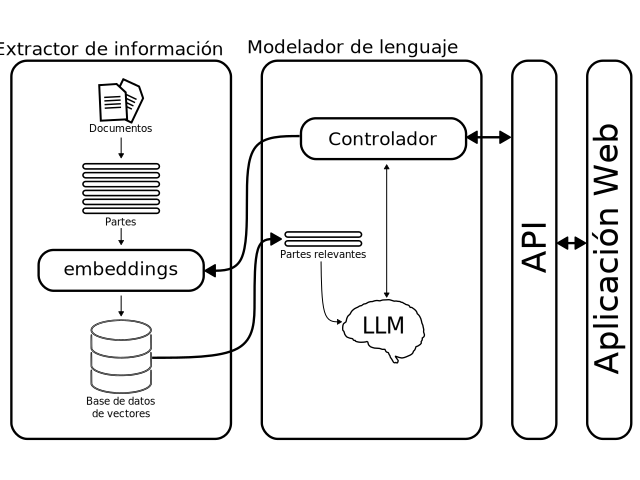
\includegraphics[width = 0.8\textwidth]{\DirFigCtres/esquema_general}
    \caption{Diagrama de componentes que conforman el sistema.}
    \label{fig:esquema_general}
\end{figure}

Para el desarrollo y puesta en producción de este proyecto se cuenta con
una estación de trabajo \textit{Dell Precission 7920 Tower} con un procesador
\textit{Intel\textregistered Xeon\textregistered Silver 4214R @2.40Ghz}, 256 GB de RAM
DDR5, un disco SSD \textit{Samsung PM881 SATA 52 GB}, un disco SSD
\textit{ADATA SU800 1TB}, dos GPUs \textit{Nvidia Quadro P620} de 2 GB de VRAM,
una GPU \textit{Nvidia RTX A4000} de 16 BG de VRAM y con sistema operativo
Windows 11. Además, se obtuvo acceso durante tres meses al centro de
supercómputo del CIMAT, a través de la convocatoria
\textit{Supercómputo como motor de colaboraciones académia-industria 2025},
para usar un nodo de cómputo GPU con dos GPUS \textit{Nvidia TITAN RTX}
de 24 GB de VRAM cada una, con Ubuntu 22.04.5. Por último, se cuenta con una laptop de desarrollo
\textit{Dell G3 15} con una GPU \textit{Nvidia GTX 1050Ti} de 4 GB de VRAM y
con Ubuntu 24.04.02.

\section{Fuente de información}

El sistema está diseñado para responder preguntas de la normativa de la
Universidad de Guanajuato, esta normativa se encuentra disponible en la página
oficial de la universidad\footnote{https://www.ugto.mx/gacetauniversitaria/normatividad/normatividad-vigente}
en forma de 22 documentos PDF individuales. Cada documento tiene un número
diferente de páginas, las cuales suman 511, representan 6.8 MB de información y,
convertidas a texto, 168,011 palabras. Para alimentar la base de datos,
los documentos son descargados manualmente y almacenados en un directorio,
donde se utiliza el nombre del archivo como identificador. En la tabla \

\begin{table}[!ht]
    \centering
    \begin{tabular}{|c|l|r|r|}
        \hline
        N  & Nombre del documento                   & Artículos & Transitorios \\ \hline
        1  & Código de Conducta e Integridad ...    & 13        & 2            \\ \hline
        2  & Código de Ética de las Personas ...    & 7         & 1            \\ \hline
        3  & Código de Ética de la Universidad ...  & NA        & 1            \\ \hline
        4  & Estatuto Orgánico de la ...            & 91        & 8            \\ \hline
        5  & Ley Orgánica de la Universidad ...     & 75        & 8            \\ \hline
        6  & Reglamento Académico de la ...         & 101       & 11           \\ \hline
        7  & Reglamento de Becas, Apoyos y ...      & 39        & 5            \\ \hline
        8  & Reglamento de Bienes del ...           & 28        & 6            \\ \hline
        9  & Reglamento de Distinciones ...         & 21        & 4            \\ \hline
        10 & Reglamento de la Defensoría de ...     & 42        & 8            \\ \hline
        11 & Reglamento de la Junta Directiva ...   & 38        & 0            \\ \hline
        12 & Reglamento del Personal Académico ...  & 98        & 7            \\ \hline
        13 & Reglamento del Programa de ...         & 38        & 4            \\ \hline
        14 & Reglamento de Mecanismos Alternos ...  & 37        & 5            \\ \hline
        15 & Reglamento de Quienes Integran ...     & 31        & 9            \\ \hline
        16 & Reglamento de Responsabilidades ...    & 53        & 7            \\ \hline
        17 & Reglamento de Transparencia y ...      & 52        & 3            \\ \hline
        18 & Reglamento Editorial de la ...         & 35        & 1            \\ \hline
        19 & Reglamento Interno del Patronato ...   & 17        & 2            \\ \hline
        20 & Reglamento para la Incorporación ...   & 49        & 5            \\ \hline
        21 & Reglamento de Responsabilidades ...    & 30        & 11           \\ \hline
        22 & Modelo Educativo de la Universidad ... & NA        & NA           \\ \hline
    \end{tabular}
    \caption{Resumen de documentos normativos de la Universidad de Guanajuato}
    \label{tab:documentos}
\end{table}

\section{Extractor de información}

El funcionamiento del módulo de extracción de información comienzan con un
archivo en formato PDF y terminan con la creación de una base de datos de
embeddings de los fragmentos del documento. En la figura
\ref{fig:esquema_extractor} se observa la secuencia de procesamiento para un
archivo y la salida de cada una de las etapas.

\begin{figure}
    \centering
    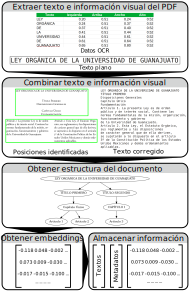
\includegraphics[width = 0.8\textwidth]{\DirFigCtres/esquema_extractor}
    \caption{Diagrama de extracción de información de un archivo PDF.}
    \label{fig:esquema_extractor}
\end{figure}

\subsection{Extraer texto e información visual del PDF}

Cada documento PDF debe convertirse a texto para su procesamiento,
conservando la información del formato y ubicación de los bloques de texto con el fin de
poder extraer la estructura de títulos y secciones del documento. Por lo anteror,
se extraen dos tipos de datos del archivo: texto plano e información visual
relacionada con el formato.

Para seleccionar las herramientas de extracción de texto plano se hizo un
análisis de aquellas que fueran de código abierto, considerando sus
deficiencias en la extracción de texto (ver Apéndice A). Se seleccionó
\textit{PyPDF}, porque es la herramienta más usada para esta tarea con Python, y
\textit{PdfPlumber}, porque su extracción de texto es la más limpia y provee mecanismos
para extraer la información visual.

Primero, se extrae el texto plano con \textit{PyPDF} o \textit{PdfPlumber}. En el caso de PyPDF
no se puede obtiener información visual que ayude a identificar los títulos, secciones
y encabezados, además en ocasiones modifica el orden del texto. Para solucionar
estos problemas se utiliza la herramienta \textit{Tesseract}, la cual es un software de
reconocimiento óptico de caracteres (OCR, Optical Character Recognition)
que permite obtener la posición, ancho, alto y texto de
cada palabra dentro del documento (Figura \ref{fig:visual_info}). Para emplear Tesseract, primero se convierte el
documento a imágenes con una densidad de pixeles de 1000 DPI con \textit{PDF2Image}, para
posteriormente procesar cada imagen con la librería \textit{PyTesseract}.
Por otra parte, cuando se usa \textit{PdfPlumber}, el texto va acompañado de la información
visual necesaria, por lo que no es necesario emplear otras herramientas.

\begin{figure}
    \centering
    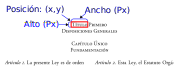
\includegraphics[width = 0.8\textwidth]{\DirFigCtres/visual_info}
    \caption{Ejemplo de información visual obtenida por \textit{Tesseract} y
        \textit{Pdfplumber}.}
    \label{fig:visual_info}
\end{figure}


\textit{Tesseract} es una herramienta, desarrollada por \textit{Google}, que puede reconstruir
el texto del documento, así como detectar las líneas, párrafos y secciones,
sin embargo, con frecuencia comete errores en la detección del texto y el
ordenamiento. Para corregir estos errores se opta por combinar el texto
plano obtenido con \textit{PyPDF}, con la información de posición y tamaño devuelta
por \textit{Tesseract}, de esta forma se obtiene el texto correcto asociado a su
ubicación y tamaño. Este proceso se describe en el diagrama de la figura
\ref{fig:texto_y_ocr}.

\begin{figure}[]
    \centering
    \includegraphics[width = 0.8\textwidth]{\DirFigCtres/esquema_texto_y_ocr}
    \caption{Detalle extracción de texto y características de OCR.}
    \label{fig:texto_y_ocr}
\end{figure}

Para el caso de PdfPlumber, la librería devuelve las mismas características que
PyTesseract, sin embargo, comete también errores en la agrupación y el
ordenamiento del texto, por ello se requiere realizar los pasos de ``Crear
grupos para reconstruir el texto'' y ``Reconstruir texto'' del diagrama de la figura
\ref{fig:texto_y_ocr}.

La tarea de agrupar el texto en secciones para reconstruirlo en el orden correcto
no es trivial, y es altamente dependiente del tipo de documento a procesar.
Este proceso se explica en los diagramas de las figuras
\ref{fig:reconstruccion_texto_1} y \ref{fig:reconstruccion_texto_2}, y
funciona adecuadamente para documentos donde predomina el texto en una o dos
columnas con títulos centrados, pero podría fallar cuando la estructura del
documento difiera considerablemente.

\begin{figure}[]
    \centering
    \includegraphics[width = 0.8\textwidth]{\DirFigCtres/reconstruccion_texto_ocr_1}
    \caption{Detalle de reconstrucción de texto del documento (Pt. 1).}
    \label{fig:reconstruccion_texto_1}
\end{figure}

\begin{figure}[]
    \centering
    \includegraphics[width = 0.8\textwidth]{\DirFigCtres/reconstruccion_texto_ocr_2}
    \caption{Detalle de reconstrucción de texto del documento (Pt 2).}
    \label{fig:reconstruccion_texto_2}
\end{figure}

Una vez realizada la agrupación de los elementos de la página, es posible reconstruir
el texto respetando el orden normal de lectura, eliminando los errores de
posicionamiento de \textit{PyPDF} o \textit{PdfPlumber} según sea el caso.
Cuando se utiliza \textit{PyPDF}+\textit{Tesseract}, el texto contiene
errores de detección que serán corregidos al combinar la información
visual del texto reconstruido, con el texto plano extraído con \textit{PyPDF}.

\subsection{Combinar texto e información visual}

Cuando se usa \textit{PdfPlumber}, este proceso no es necesario, pues la librería ya
devuelve el texto correcto asociado a su información visual de posición y tamaño,
sin embargo, cuando se usa \textit{PyPDF}+\textit{PyTesseract}, es necesario combinar estas dos
fuentes de información para obtener el texto y la información visual correctas.
El objetivo es tener la posición de cada palabra asociada con su texto correcto,
de esta forma se podrá distinguir entre diferentes elementos, como títulos,
párrafos, entre otros.

El proceso de combinación requiere las cadenas de texto extraídas por los dos métodos:
la cadena proporcionada por \textit{PyPDF} y la cadena reconstruida con la información
visual, como se muestra en la figura \ref{fig:reconstruccion_texto_2}. Ambas cadenas se
separan por palabra y se pasan a la librería \textit{Difflib}, la cual aplica el algoritmo
Ratcliff-Obershelp, también conocido como Coincidencia de patrones Gestalt, para
comparar dos cadenas y encontrar sus diferencias.

Si se analizan los patrones de salida de la librería \textit{Difflib}, es posible
corregir las palabas detectadas con OCR utilizando las palabras extraídas directamente
del texto, los detalles de esta implementación se explican en la figura
\ref{fig:esquema_combinacion_txt_ocr}.
En escencia, se considera la palabra obtenida con \textit{PyPDF} como la correcta,
se compara contra la palabra obtenida con \textit{Tesseract} y si es diferente se sobreescribe.
Al terminar el proceso se tiene un arreglo de datos donde se conoce la posición
y dimensiones de cada palabra, así como su texto correcto, además se cuenta con
datos adicionales de línea, columna, alineación o grupo que serán empleadas
para dividir las secciones del documento más adelante.


\begin{figure}[]
    \centering
    \includegraphics[width = 0.8\textwidth]{\DirFigCtres/combinacion_texto_ocr}
    \caption{Detalle de combinación de texto plano con información de OCR.}
    \label{fig:esquema_combinacion_txt_ocr}
\end{figure}

Las ventajas de usar \textit{PdfPlumber} sobre \textit{PyPDF}+\textit{PyTesseract}
son que \textit{PdfPlumber} es más rápido y
la identificación del texto es certera, pues proviene directamente del archivo,
sin embargo, no funciona si el PDF es un escaneo o si contiene texto en forma
de imagen. Por su parte, al generar el método de \textit{PyPDF}+\textit{PyTesseract}, se desarrollaron
elementos que fueron reutilizados al usar \textit{PdfPlumber}, como la resconstrucción de texto.
Además, si se confía plenamente en la predicción de \textit{PyTesseract}, se
puede dar soporte a documentos escaneados o con imágenes con texto.

\subsection{Obtener estructura del documento}

El objetivo de este paso es generar una estructua de datos en la que cada parte
del documento esté referenciada a su sección y subsecciones correspondientes,
por ejemplo, para la Ley Orgánica se desea conocer en qué título, capítulo y
artículo se encuentra un texto específico. Para crear dicha estructura, se optó por generar un árbol, donde cada nodo
corresponde a una sección del documento, además, las hojas y los nodos intermedios
almacenan el texto de cada artículo o sección según sea el caso. En la figura
\ref{fig:fragmento_arbol} se muestra un fragmento del árbol correspondiente a
las primeras secciones de la Ley Orgánica.

\begin{figure}[]
    \centering
    \includegraphics[width = 0.8\textwidth]{\DirFigCtres/fragmento_arbol}
    \caption{Fragmento de árbol de documento ``Ley Orgánica de la Universidad de Guanajuato''.}
    \label{fig:fragmento_arbol}
\end{figure}

Para generar el árbol es necesario analizar el documento en varios pasos. Primero,
se detectan las líneas o segmentos que corresponden a títulos, estas típicamente
se encuentran centrados en la página o en la columna, además de presentar un
espacio vertical antes o después. Para encontrar las secciones o subsecciones
se consideran los títulos centrados en la página y se les asigna un nivel.
Para asignar el nivel se debe conocer de antemano la estructura del documento
y generar expresiones regulares que ayuden a diferenciar un título, de un subtítulo,
y así sucesivamente. Para los documentos normativos de la Universidad
de Guanajuato la estructura es la siguiente:

\begin{enumerate}
    \item \textbf{Encabezado general:} Son textos abiertos que no tienen palabras o
          estructura específica y se consideran dentro del primer nivel.
          \begin{itemize}
              \item Sin expresión regular
          \end{itemize}
    \item \textbf{Título:} Los documentos se dividen en títulos. Cada título comienza con
          la palabra \textit{Título}. También pueden ser numerales romanos.
          \begin{itemize}
              \item \string^(título\textbar[xiv]+\textbackslash.) .*
          \end{itemize}
    \item \textbf{Sección (Opcional):} Algunos documentos dividen los títulos en secciones.
          Cada sección comienza con la palabra \textit{Sección}. También pueden ser
          secciones numeradas.
          \begin{itemize}
              \item \string^([0-9]+\.[0-9]|sección) .*
          \end{itemize}
    \item \textbf{Capítulo:} Los títulos o secciones se dividen en capítulos y cada capítulo comienza
          con la palabra \textit{Capítulo}
          \begin{itemize}
              \item \string^capítulo .*
          \end{itemize}
\end{enumerate}

Además, se debe tener en cuenta que hay divisiones del documento
que no se encuentran centrados, sino que están contenidos en el grueso del
texto, como lo son los Artículos. Para identificar estas separaciones en el
contenido, también se crean expresiones regulares que se verifican contra el
inicio de cada línea mientras se va construyendo el árbol.

\begin{enumerate}
    \item \textbf{Artículo:} Los capítulos tienen uno o más artículos.
          \begin{itemize}
              \item  \string^artículo ([0-9]+\textbar[a-zé]+(ro\textbar do\textbar ro\textbar to\textbar mo\textbar vo\textbar no\textbar único)\\
                    (bis\textbar ter\textbar quáter\textbar quinquies)?\textbackslash.
          \end{itemize}
\end{enumerate}

Una vez identificados los títulos y teniendo la forma para encontrar las
divisiones dentro del contenido, se recorre el documento. Recorrer
el documento es el equivalente a recorrer el árbol por profundidad, por lo
que se va creando el árbol de la misma forma, es decir, cuando se encuentra
un título se crea un nuevo nodo en el nivel correspondiente, siempre teniendo
la referencia de cual será su padre, cuando se llega al nivel más bajo se
guarda el contenido de texto en el nodo correspondiente.
El proceso completo se presenta en la figura
\ref{fig:crear_arbol}.

\begin{figure}[]
    \centering
    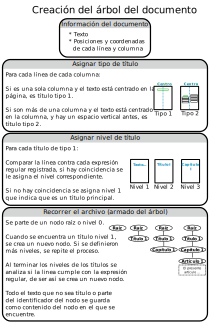
\includegraphics[width = 0.8\textwidth]{\DirFigCtres/crear_arbol}
    \caption{Proceso de creación del árbol de secciones de un documento.}
    \label{fig:crear_arbol}
\end{figure}

\subsection{Obtener \textit{embeddings}}

Para el cálculo de \textit{embeddings} se emplean modelos LLM de extracción de
\textit{embeddings}. El sistema propuesto permite el uso y evaluación de
varios modelos, los cuales serán: MiniLM (33M de parámetros)
\cite{wang_minilm_2020}, MPNET \cite{hagen_mpnet_2020} (110M de parámetros)
y Qwen 3 \cite{zhang_qwen3_2025} (600M, 4B y 8B de parámetros). Estos modelos
se encuentran disponibles en HuggingFace y se pueden
usar con las librearías \textit{SentenceTransformers} o \textit{Transformers}.

Los modelos MiniLM y MPNET fueron seleccionados por su tamaño reducido,
ya que pueden ejecutarse en CPU de forma eficiente. Los
modelos Qwen se seleccionaron ya que ocupan los primeros puestos en el
MTEB Ladderboard de HuggingFace\footnote{https://huggingface.co/spaces/mteb/leaderboard},
que clasifica modelos de extracción de \textit{embeddings} en diferentes idiomas
y con múltiples métricas. Además, con el objetivo de reducir el uso de memoria,
también se evalúan los modelos
cuantizados de Qwen 3: f16 (16 bits), Q8\_0 (8 bits), Q6\_K (6 bits), Q5\_K\_M (5 bits)
y Q4\_K\_M (4 bits). Estos modelos cuantizados se emplean con la librería \textit{llama\_cpp},
la cual es una implementación de la arquitectura \textit{Llama} de Meta en
C/C++ para hacer inferencia de forma eficiente. Un resumen de las características
de los modelos de extracción de \textit{embeddings} se encuentra en la tabla \ref{tab:embed_models}.

\begin{table}[!ht]
    \centering
    \begin{tabularx}{0.8\textwidth}{|l|l|r|X|}
        \hline
        Modelo                     & Tipo de dato & Memoria  & Tamaño Embed. \\ \hline
        Qwen3-Embedding-0.6B       & BF16         & 3.65 GB  & 1024          \\ \hline
        Qwen3-Embedding-4B         & BF16         & 15.31 GB & 2560          \\ \hline
        Qwen3-Embedding-8B         & BF16         & 28.5 GB  & 4096          \\ \hline
        Qwen3-Embedding-0.6B-GGUF  & Q8\_0        & 2.51 GB  & 1024          \\ \hline
        Qwen3-Embedding-0.6B-GGUF  & F16          & 3.03 GB  & 1024          \\ \hline
        Qwen3-Embedding-4B-GGUF    & Q4\_K\_M     & 5.01 GB  & 2560          \\ \hline
        Qwen3-Embedding-4B-GGUF    & F16          & 10.18 GB & 2560          \\ \hline
        Qwen3-Embedding-8B-GGUF    & Q4\_K\_M     & 7.05 GB  & 4096          \\ \hline
        Qwen3-Embedding-8B-GGUF    & F16          & 16.82 GB & 4096          \\ \hline
        all-MiniLM-L6-v2           & I64/F32      & 144 MB   & 384           \\ \hline
        multi-qa-mpnet-base-dot-v1 & I64/F32      & 478 MB   & 768           \\ \hline
    \end{tabularx}
    \caption{Resumen de modelos de extracción de \textit{embeddings}}
    \label{tab:embed_models}
\end{table}

El proceso para convertir la información del documento a embeddings consiste
en recorrer el árbol en profundidad, y en cada nodo hacer lo siguiente:

\begin{enumerate}
    \item Tomar el contenido textual del nodo, separarlo por párrafos y
          agrupar los párrafos en fragmentos de aproximadamente C caracteres.
          Cada fragmento será un registro independiente.
    \item Utilizar \textit{SentenceTransformers}/\textit{Transformers}/\textit{Llama\_cpp}
          para calcular el \textit{embedding} de cada fragmento y guardarlo como un vector de números.
    \item Obtener la ruta del nodo dentro del árbol. Ej: Ley Orgánica $\rightarrow$
          Título Primero $\rightarrow$ Capítulo segundo $\rightarrow$ Artículo 30.
    \item Guardar la ruta y el nombre del nodo como metadatos, así como el nombre
          del documento y cualquier información relevante.
\end{enumerate}

Al final, por cada fragmento del documento se tendrá la siguiente información:

\begin{itemize}
    \item Texto del fragmento.
    \item \textit{Embedding} como vector de N valores numéricos.
    \item Metadatos:
          \begin{itemize}
              \item Nombre del documento.
              \item Ruta en el árbol.
              \item Nombre del nodo.
              \item Número de fragmento dentro del nodo.
              \item Nombre del nodo padre
          \end{itemize}
\end{itemize}

\subsection{Almacenar información}

Los \textit{embeddings} pueden almacenarse de varias formas en el disco siendo, las más
convenientes el formato CSV y las bases de datos con soporte para vectores.
El formato CSV tiene la ventaja de ser portable y fácil de leer, basta con
convertir los metadatos a formato JSON, para que puedan ser almacenados
como texto, mientras que el vector de \textit{embedding} se puede
expandir y crear una columna para cada valor. En la figura \ref{fig:ejemplo_csv}
se muestra un ejemplo de la información almacenada como archivo CSV.
Este método funciona bien para hacer la evaluación y análisis de los modelos,
sin embargo, no es apto para entornos productivos, ya que no se tienen
optimizados para la búsqueda en los vectores de datos.

\begin{figure}[]
    \centering
    \includegraphics[width = 0.8\textwidth]{\DirFigCtres/ejemplo_csv}
    \caption{Ejemplo almacenamiento de metadatos y \textit{embeddings} en formato csv.}
    \label{fig:ejemplo_csv}
\end{figure}

Otra forma de almacenar los \textit{embeddings} es empleando una base de datos que
soporte vectores. El mayor beneficio de estas herramientas es que
permiten almacenar los datos de forma óptima, ya que la información
se puede agrupar en tablas, se puede agregar información adicional y
cuentan con funciones optimizadas de búsqueda por similitud de vectores.
Algunos ejemplos de estas bases de datos vectoriales son: Chroma, Marco o
PostgreSQL.

Este proyecto emplea ChromaDB, la cual funciona con SQLite y está diseñada para funcionar en
entornos productivos, e incluye mecanismos para calcular los embeddings
empleando \textit{SentenceTransformers} u otro método personalizado, además,
permite el uso de diferentes parámetros de búsqueda por similitud semántica
como son la distancia coseno y el producto interno, los cuales también se
encuentran optimizados. En la figura \ref{fig:ejemplo_chromadb} se muestra
un ejemplo de datos almacenados en ChromaDB.

\begin{figure}[]
    \centering
    \includegraphics[width = 0.8\textwidth]{\DirFigCtres/ejemplo_chromadb}
    \caption{Ejemplo de cómo se almacenan metadatos en Chroma DB. Los vectores
        se almacenan de forma óptima en un archivo separado.}
    \label{fig:ejemplo_chromadb}
\end{figure}

\section{Modelador de lenguaje}

El modelador de lenguaje tiene dos funciones fundamentales: manejar la
interacción con la base de datos de vectores y hacer uso del
LLM de inferencia principal, en términos de RAG, se encarga de la
recuperación y la generación. El proceso general que ejecuta el modelador
de lenguaje se presenta en el diagrama de la figura
\ref{fig:esquema_modelador} y se explica en las siguientes subsecciones.

\begin{figure}
    \centering
    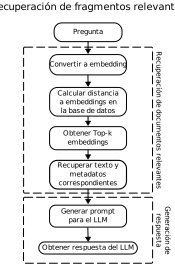
\includegraphics[width = 0.75\textwidth]{\DirFigCtres/esquema_recuperacion}
    \caption{Pasos seguidos por el modelador de lenguaje para procesar una pregunta.}
    \label{fig:esquema_modelador}
\end{figure}

\subsection{Recuperación de documentos relevantes}

Dada una pregunta, el modelador la convierte a \textit{embedding}
empleando el mismo modelo usado en la base de datos de vectores. Este \textit{embedding}
se le proporciona a ChromaDB para que realice la búsqueda semántica, el parámetro
de búsqueda puede ser por producto interno o por similitud coseno, dependiendo
del modelo de \textit{embedding}. Para hacer una búsqueda eficiente,
ChromaDB emplea un índice llamado HNSW (Hierarchical Navigable Small World),
esto le permite encontrar los fragmentos con mayor similitud sin tener que
comparar con toda la base de datos.

Con ChromaDB se obtiene el top \textit{k} de \textit{embeddings} similares,
por defecto \textit{k} se establece en 5. De estos \textit{k} \textit{embeddings}
se obtiene su texto original, su posición dentro del árbol del documento, el
documento al que pertenece y los demás metadatos.

\subsection{Generación de respuesta}

Para la generación de la respuesta, se emplea un modelo multidominio de código
abierto. Para seleccionar el modelo óptimo para el sistema se seleccionaron
distintos modelos cuya restricción principal es que pudieran ejecutarse en el
hardware del sistema, es decir, que funcionen correctamente con 16 GB de VRAM.
Se evaluarán los modelos Qwen 3 \cite{zhang_qwen3_2025} (600M y 8B de parámetros)
en sus versiones completas y cuantizadas, Llama 3.1 (8B de parámetros) en
su versión completas y el modelo GPT-OSS (20B de parámetros) en su versión
cuantizada.

\begin{table}[!ht]
    \centering
    \begin{tabular}{|l|l|l|l|l|l|}
        \hline
        Modelo                & Tipo de dato & Memoria  & Herramienta  \\ \hline
        Qwen3-0.6B            & BF16         & 1.74 GB  & Transformers \\ \hline
        Qwen3-8B              & BF16         & 15.59 GB & Transformers \\ \hline
        Qwen3-8B-Q4\_K\_M     & Q4\_K\_M     & 7.07 GB  & Llama\_cpp   \\ \hline
        gpt-oss-20b-MXFP4     & MXFP4        & 13.76 GB & Llama\_cpp   \\ \hline
        Llama-3.1-8B-Instruct & BF16         & 15.27 GB & Transformers \\ \hline
    \end{tabular}
    \caption{Resumen de modelos de generación de respuesta.}
    \label{tab:llm_models}
\end{table}

Para la evaluación inicial, a todos los modelos se les configura una instrucción
de sistema simple que le indica que su propósito es ser un asistente, esto
con el objetivo de evaluarlos en su forma básica.

\begin{verbatim}
    Eres un asistente que ayuda a responder preguntas.
\end{verbatim}

En una segunda evaluación, se comparan únicamente los mejores modelos de la primera etapa,
pero esta vez con una instrucción de sistema más compleja, donde se incluyen instrucciones
de cómo procesar las preguntas, el tono en que debe contestar, entre otros elementos.
Esta instrucción es más cercana a la que se usará en la aplicación final.

\begin{verbatim}
Eres un asistente virtual experto en la normativa de la
Universidad de Guanajuato. Tu único propósito es responder a
las preguntas de los usuarios basándote estricta y
exclusivamente en los fragmentos de los documentos normativos
que se te proporcionen en cada consulta.

**Instrucciones de Operación:**

1. **Rol y Personalidad:** Actúa como un asistente
   universitario formal, preciso y servicial. Tu tono debe ser
   siempre profesional, claro y objetivo. No uses un lenguaje
   coloquial ni opiniones personales.
2. **Fuente de Verdad:** Los documentos proporcionados en
   la sección `<contexto>` son tu única fuente de información.
   No debes usar ningún conocimiento previo que tengas sobre
   esta u otras universidades, ni información externa a la
   proporcionada.
3. **Proceso para Responder:**
   * Analiza detenidamente la pregunta del usuario en la
   sección `<pregunta>`.
   * Revisa cuidadosamente los fragmentos de texto en la
   sección `<contexto>`. Los fragmentos de texto se
   encuentran en formato JSON y contienen el nombre del
   documento, el nombre de la sección o artículo y el
   contenido del fragmento.
   * Ignora los fragmentos de texto en la sección
   `<contexto>` que no estén relacionados con la pregunta o
   en los que no esté presente la respuesta.
   * Formula una respuesta concisa y directa a la pregunta
   del usuario utilizando únicamente la información
   encontrada en el `<contexto>`.
4. **Manejo de Información Insuficiente:**
   * Si la información en el `<contexto>` no es suficiente
   para responder a la pregunta del usuario de manera
   completa y precisa, debes indicar claramente: "No he
   encontrado información suficiente en los documentos
   proporcionados para responder a tu pregunta." y solicita
   al usuario que intente de nuevo reformulando la pregunta.
   * No intentes inferir, adivinar o completar información
   que no esté explícitamente escrita en el `<contexto>`.
   Es crucial que no inventes respuestas.
5. **Formato de la Respuesta:**
   * La respuesta debe ser clara y estar redactada en un
   español impecable.
   * Utiliza viñetas o listas numeradas si ayuda a clarificar
   la información extraída de los documentos.
   * No añadas saludos, despedidas ni frases introductorias
   como "Claro, aquí tienes la respuesta:" o "Basado en la
   información...". Responde directamente a la pregunta.

**Ejemplo de cómo debes procesar la información:**

<pregunta>
{question}
</pregunta>

<contexto>
{context}
</contexto>
\end{verbatim}

Teniendo la pregunta y los fragmentos relevantes con sus metadatos,
se transmite la información al LLM a través de una instrucción con una plantilla,
que contiene la pregunta, y los documentos relevantes en formato JSON
con todos sus datos. Una vez generada la instrucción, se le proporciona
al modelo, junto con el historial anterior del chat en caso de
existir para obtener la respuesta.

\begin{verbatim}
<pregunta>
{pregunta}
<pregunta>

<contexto>
{documentos_en_JSON}
</contexto>
\end{verbatim}

\section{API de comunicación}

La tarea de la API es conectar la aplicación web con el modelador de lenguaje.
La API funciona con peticiones http de tipo POST y expone un solo endpoint
que recibe parámetros en formato JSON, además esta protegida con un API-KEY
que se debe enviar en el encabezado de cada petición. Un ejemplo de petición
se muestra en la figura \ref{fig:parametros_api}. La estructura de una petición es la siguiente:

\begin{itemize}
    \item \textbf{model:} Identificador del modelo a emplear.
    \item \textbf{num\_related\_questions:} (Opcional) Número de preguntas previas a tomar
          en cuenta para buscar documentos relevantes. Por defecto 1.
    \item \textbf{messages:} Lista de mensajes.
          \begin{itemize}
              \item \textbf{role:} Rol del mensaje. ``system'', ``user'' o ``assistant''.
              \item \textbf{content:} Texto de la pregunta, respuesta o instrucción.
          \end{itemize}
\end{itemize}

\begin{figure}[]
    \centering
    \includegraphics[width = 0.8\textwidth]{\DirFigCtres/parametros_api}
    \caption{Ejemplo de petición a API.}
    \label{fig:parametros_api}
\end{figure}

La respuesta de la API también es en formato JSON y contiene el texto de la
respuesta, así como los fragmentos de los documentos que fueron tomados como contexto para
emitirla, como se muestra en la figura \ref{fig:respuesta_api}. En estos
documentos, se incluyen los metadatos para poder desplegarlos en la aplicación
web. La estructura de la respuesta es la siguiente:

\begin{itemize}
    \item \textbf{iderror:} Identificador del error. 0 en caso de que no haya error.
    \item \textbf{msgerror:} Mensaje de error, en caso de haberlo.
    \item \textbf{choices:} Respuesta del modelo, como arreglo de respuestas, aunque
          solo sea una.
          \begin{itemize}
              \item \textbf{content:} Contenido de texto de la respuesta.
              \item \textbf{metadata:} Metadatos de los fragmentos de referencia.
                    \begin{itemize}
                        \item \textbf{title:} Título de la sección.
                        \item \textbf{path:} Ruta del fragmento en la estructura del documento.
                        \item \textbf{document\_name:} Nombre del documento de referencia.
                        \item \textbf{parent:} Nombre de la sección donde se encuentra el fragmento.
                    \end{itemize}
          \end{itemize}
\end{itemize}

\begin{figure}
    \centering
    \includegraphics[width = 0.8\textwidth]{\DirFigCtres/respuesta_api}
    \caption{Ejemplo de respuesta de API.}
    \label{fig:respuesta_api}
\end{figure}

\section{Aplicación web}

La aplicación web es la única fuente de interacción de los usuarios con el
sistema, es por ello que debe contener todas las funcionalidades necesarias
que en este caso son: ingresar una pregunta, recibir una respuesta y
consultar los documentos que dan fundamento a dicha respuesta. Bajo esta
la aplicación web debe contar con una caja de texto para hacer la pregunta
y un mecanismo para mostrar la lista de mensajes y respuestas como un chat
convencional. Adicionalmente, se debe destinar un espacio para colocar los
documentos relacionados con la pregunta, como se muestra en el
\textit{wireframe} de la figura \ref{fig:wireframe_chat}.

\begin{figure}
    \centering
    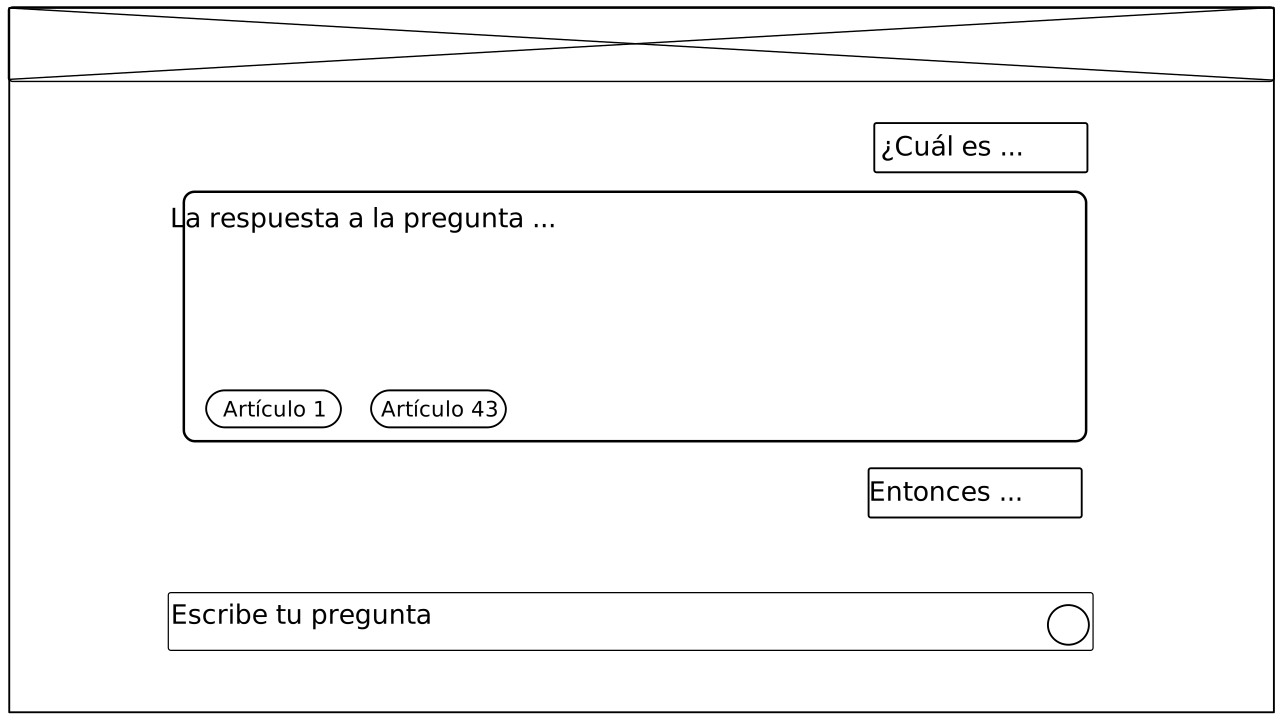
\includegraphics[width = 0.8\textwidth]{\DirFigCtres/wireframe_chat}
    \caption{Esqueleto del chat de la aplicación.}
    \label{fig:wireframe_chat}
\end{figure}

\section{Evaluación de los modelos}

Para seleccionar los modelos de extracción de \textit{embeddings} y de
inferencia más aptos, se realiza una evaluación en varios pasos, donde de cada paso
se seleccionan los mejores modelos, hasta llegar a la mejor combinación
considerando rendimiento y recursos.

\subsection{Conjunto de datos de evaluación}

Es necesario generar un conjunto de datos de preguntas y respuestas
relacionadas con los documentos normativos, para conocer el rendimiento
de los modelos en este dominio específico.
Tres personas fungen como los generadores de preguntas, a cada una se le
proporcionan 7 u 8 documentos, para completar el total de 21, se
excluye el documento denominado ``Modelo Educativo de la Universidad
de Guanajuato y su Modelo Académico'' pues no se encuentra divido en
artículos y dificultaría la referenciación de las respuestas. Se instruye a cada
participante para que genere de 1 a 4 preguntas por cada artículo de cada
documento, ignorando los textos introductorios. Cada pregunta debe
contener la siguiente información: pregunta, respuesta y contexto.
La pregunta debe redactarse de forma natural, mientras que la respuesta debe encontrarse
directamente en el artículo correspondiente del documento y debe ser copiada
directamente del mismo, por último, el contexto corresponde al nombre del
artículo de donde fue extraída la pregunta.

La base de datos se genera en formato CSV, por conveniencia de los
participantes, pero después se convierte a JSON y complementa con
otros campos relevantes para que sea similar a la estructura del
conjunto de datos SQuAD. Posteriormente, el conjunto de datos es
a la plataforma HuggingFace como un dataset de QA por conveniencia.
Una entrada del dataset final contiene los siguientes elementos:

\begin{itemize}
    \item \textbf{id:} Identificador único de la pregunta. Es un MD5.
    \item \textbf{title:} Nombre del documento.
    \item \textbf{context:} Nombre del artículo donde se encuentra la respuesta.
    \item \textbf{context\_text:} Texto plano del artículo donde se encuentra la respuesta.
    \item \textbf{additional\_context:} En caso de que el artículo haga referencia a otro documento o artículo se incluye aquí.
    \item \textbf{question:} Texto de la pregunta.
    \item \textbf{anwers:}
          \begin{itemize}
              \item \textbf{text:} Arreglo con las cadenas de respuesta a la pregunta. Usualmente solo es una.
          \end{itemize}
\end{itemize}

\subsection{Evaluación del modelo de \textit{embedding}}

El objetivo de esta evaluación es conocer la calidad de los documentos
identificados como relevantes para cada una de las preguntas del conjunto de
datos. Se emplearán tres métricas: \textit{precision@k}, \textit{recall@k} y
\textit{f1@k}. Cada una de estas métricas se definen con las ecuaciones
\ref{eq:precision}, \ref{eq:recall}, \ref{eq:f1} respectivamente. Para
aplicar las fórmulas \ref{eq:precision} y \ref{eq:recall}, se considera
como fragmento relevante a aquel que su nombre del nodo, coincida con el
nombre del artículo donde se encuentra la respuesta (\textit{context}
en el conjunto de datos).

\begin{equation}\label{eq:precision}
    \text{precision@k} = \frac{\text{N fragmentos relevantes en top k}}{k}
\end{equation}

\begin{equation}\label{eq:recall}
    \text{recall@k} = \frac{\text{N fragmentos relevantes en top k}}{\text{N fragmentos relevantes totales}}
\end{equation}

\begin{equation}\label{eq:f1}
    \text{f1@k} = \frac{2 \times \text{precision} \times \text{recall}}{\text{precision} + \text{recall}}
\end{equation}

El proceso de evaluación de los embeddings se realiza siguiendo los siguientes
pasos:

\begin{enumerate}
    \item Para cada pregunta, se identifican los fragmentos relevantes reales. Es decir,
          los fragmentos del artículo donde se encuentra la respuesta.
    \item Se calcula la similitud coseno entre la pregunta y cada fragmento de
          la base de datos de \textit{embeddings}, incluyendo todos los documentos.
    \item Se obtienen los k fragmentos con mayor similitud coseno.
    \item Se calculan las métricas de evaluación con los k fragmentos obtenidos.
    \item El proceso se repite con todas las preguntas del conjunto de datos y
          al final se obtienen las medias de cada métrica.
\end{enumerate}

\subsection{Evaluación del modelo de inferencia}

El objetivo de esta evaluación es conocer la similitud de la respuesta
dandidata con la respuesta de referencia, y si la respuesta responde correctamente
la pregunta. Se emplearán tres métricas principales: puntuación ROUGE,
puntuación BERT y similitud coseno. ROUGE (Recall-Oriented Understudy for
Gisting Evaluation) es una métrica que evalúa la superposición entre una
oración candidata y otra de referencia, en específico, ROUGE-L emplea la
subsecuencia de texto en común más larga (LCS, Longest Common Subsequence)
para calcular la precisión, recall y la puntuación f1, como se muestra en
las fórmulas \ref{eq:precision_lcs}, \ref{eq:recall_lcs}, \ref{eq:f1_lcs}.

\begin{equation}\label{eq:precision_lcs}
    P_{LCS} = \frac{\text{N palabras en LCS}}{\text{N palabras en respuesta inferida}}
\end{equation}

\begin{equation}\label{eq:recall_lcs}
    R_{LCS} = \frac{\text{N palabas en LCS}}{\text{N palabras en referencia}}
\end{equation}

\begin{equation}\label{eq:f1_lcs}
    F1_{LCS} = \frac{2 \times P_{LCS} \times R_{LCS}}{P_{LCS} + R_{LCS}}
\end{equation}

La puntuación BERT consiste en tomar la respuesta candidata y la respuesta
de referencia, tokenizarla y obtener el \textit{embedding} de cada token con un modelo BERT.
Una vez obtenidos los \textit{embeddings}, se calcula la similitud coseno entre
cada token de la secuencia candidata $(\hat{x}_1, ..., \hat{x}_k)$ y cada
token de la referencia $(x_1, ..., x_m)$, para calcular la precisión y recall
empleando los tokens más similares, como se muestra en las ecuaciones
\ref{eq:precision_bert}, \ref{eq:recall_bert} y \ref{eq:f1_bert}.

\begin{equation}\label{eq:precision_bert}
    P_{BERT} = \frac{1}{|\hat{x}|}\sum_{\hat{x}_j \in \hat{x}}\max_{x_i \in x}x_i^T \hat{x}_j
\end{equation}

\begin{equation}\label{eq:recall_bert}
    R_{BERT} = \frac{1}{|x|}\sum_{x_i \in x}\max_{\hat{x}_j \in \hat{x}}x_i^T \hat{x}_j
\end{equation}

\begin{equation}\label{eq:f1_bert}
    F1_{BERT} = \frac{2 \times P_{BERT} \times R_{BERT}}{P_{BERT} + R_{BERT}}
\end{equation}

Por último, la similitud coseno se evalua calculando el \textit{embedding}
de la respuesta candidata y el de la respuesta referencia, para ello
se emplea un modelo simple de extracción de \textit{embeddings} como
el all-MiniLM-L6-v2 y se obtiene la similitud coseno entre ambos vectores.

\section{Reentrenamiento del modelo de \textit{embeddings}}

En este proyecto se emplea la forma más directa de reentrenamiento o ajuste
fino, que es el reentrenamiento completo del modelo sobre un conjunto
de datos sepecializados. El conjunto de datos será el descrito anteriormente
para la evaluación de los modelos, haciendo una división aleatoria de 80\%
de muestras para el entrenamiento y un 20\% para la evaluación. Esta
separación se hace a nivel archivo, por lo que se garantiza que haya al menos
exista una pregunta de cada documento.

Para reentrenar se emplea la librería \textit{SentenceTransformers}, la
cual permite cargar un modelo y reentrenarlo con una función de pérdida
específica, dependiendo de la tarea. En este caso, la función de pérdida
es \textit{CachedMultipleNegativesRankingLoss}, que requiere pares de oraciones
(ancla, positivo) o tríos (ancla, positivo, negativo) para maximizar la
similitud entre el ancla y la secuencia positiva. Para generar estos pares
de oraciones, se considera cada muestra del conjunto de datos original y
se emplea la pregunta como el ancla, el texto del contexto como el par
positivo, y texto del contexto de otra pregunta como la parte negativa.
Se harán pruebas de entrenamiento con solamente ancla y positivo, así como
pruebas con el texto negativo también. Dadas las limitaciones del hardware,
solamente se hará reentrenamiento sobre los modelos all-MiniLM-L6-v2 y el
multi-qa-mpnet-base-dot-v1 por su tamaño reducido.
